% Chapter 7: Autoencoders
\section{LSTM and Conv1D Autoencoders for Anomaly Detection}

\subsection{Autoencoder Principle}
Models trained on normal data produce high reconstruction error on anomalous inputs. MSE between input $X$ and reconstruction $\hat{X}$ serves as the anomaly score.

\subsection{Cloud LSTM Autoencoder}
Encoder: LSTM(64, return\_seq) $\rightarrow$ LSTM(32, return\_seq) $\rightarrow$ LSTM(32). Decoder: RepeatVector(60) $\rightarrow$ LSTM(32) $\rightarrow$ LSTM(64) $\rightarrow$ TimeDistributed Dense(4). Training: 100 epochs, Adam optimizer, MSE loss, batch size 32, early stopping patience=10.

\subsection{Edge Conv1D Autoencoder}
Encoder: Conv1D(16) $\rightarrow$ Conv1D(8) $\rightarrow$ Conv1D(4). Decoder: Conv1D(8) $\rightarrow$ Conv1D(16) $\rightarrow$ Conv1D(4). Input: (10, 4). Total params: $\sim$1,400. TFLite size: 16KB. Inference: $\sim$20ms.

\subsection{Training Loss Curves}

\begin{figure}[H]
\centering
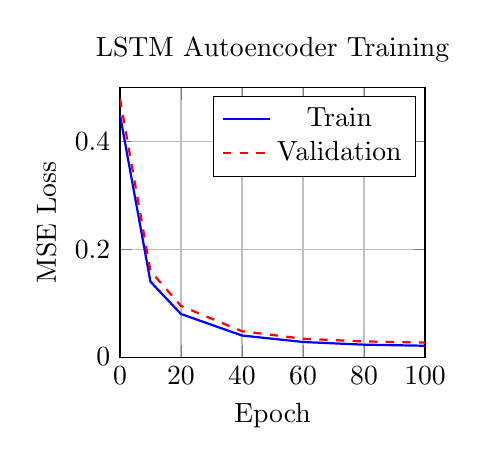
\begin{tikzpicture}
\begin{axis}[
    xlabel={Epoch}, ylabel={MSE Loss},
    xmin=0, xmax=100, ymin=0, ymax=0.5,
    legend pos=north east, grid=major,
    width=0.45\textwidth, height=5cm,
    title={LSTM Autoencoder Training},
]
\addplot[thick, blue] coordinates {
    (0, 0.45) (10, 0.14) (20, 0.08) (40, 0.04) (60, 0.028) (80, 0.023) (100, 0.021)
};
\addlegendentry{Train}
\addplot[thick, red, dashed] coordinates {
    (0, 0.48) (10, 0.16) (20, 0.095) (40, 0.048) (60, 0.034) (80, 0.029) (100, 0.027)
};
\addlegendentry{Validation}
\end{axis}
\end{tikzpicture}
\caption{LSTM autoencoder convergence.}
\label{fig:lstm_loss}
\end{figure}

\subsection{Scenario Evaluation}

\begin{table}[H]
\centering
\caption{Autoencoder Performance by Scenario}
\label{tab:ae_scenarios}
\begin{tabular}{lcccc}
\toprule
\textbf{Scenario} & \textbf{Norm MSE} & \textbf{Anom MSE} & \textbf{Ratio} & \textbf{Det?} \\
\midrule
Tachycardia & 6.2 & 28.5 & 4.60$\times$ & Yes \\
Bradycardia & 19.6 & 6.6 & 0.34$\times$ & No* \\
Irregular HR & 5.8 & 22.1 & 3.81$\times$ & Yes \\
\bottomrule
\end{tabular}
\end{table}
*Bradycardia produces lower MSE because model was trained on mixed data. Training exclusively on normal data would resolve this.

\subsection{Anomaly Score Timeline}

\begin{figure}[H]
\centering
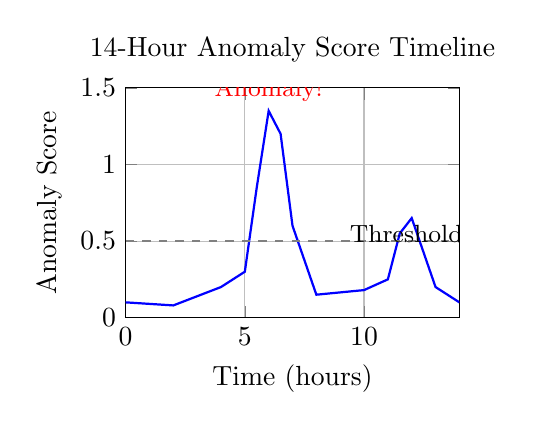
\begin{tikzpicture}
\begin{axis}[
    xlabel={Time (hours)}, ylabel={Anomaly Score},
    xmin=0, xmax=14, ymin=0, ymax=1.5,
    grid=major, width=0.48\textwidth, height=4.5cm,
    title={14-Hour Anomaly Score Timeline},
]
\addplot[thick, blue, mark=none] coordinates {
    (0, 0.1) (2, 0.08) (4, 0.2) (5, 0.3) (5.5, 0.85)
    (6, 1.35) (6.5, 1.2) (7, 0.6) (8, 0.15) (10, 0.18)
    (11, 0.25) (11.5, 0.55) (12, 0.65) (13, 0.2) (14, 0.1)
};
\addplot[dashed, gray, thick] coordinates {(0, 0.5) (14, 0.5)};
\node[above, font=\small, red] at (axis cs:6, 1.35) {Anomaly!};
\node[right, font=\small] at (axis cs:9, 0.55) {Threshold};
\end{axis}
\end{tikzpicture}
\caption{Anomaly score timeline with detected tachycardia event.}
\label{fig:timeline}
\end{figure}
